

%!TEX root = ../dissertation.tex
\chapter{FUNCTIONAL DATA ANALYSIS APPROACH TO LAND COVER CLASSIFICATION IN INDIA USING MERIS TERRESTRIAL CHLOROPHYLL INDEX} \label{phenology}

\section{Introduction}

Phenology is the study of annual life-cycles of terrestrial vegetation and how they are effected by climate change or other environmental variables. Understanding vegetation phenology and its spatio-temporal variation is required to reveal and predict ongoing changes in Earth system dynamics (\cite{Jeganathan:2010gqa}). While ground based phenological measurements can provide information on specific species with high temporal resolution it is challenging to get rich spatial information (\cite{Studer:2007hd}). Monitoring phenology at the ground level also suffers from subjectivity, and a difficulty to relate field data with climatic variables (\cite{Jeganathan:2010gqa}). Remotely sensed data, on the other hand, can provide spatial information at local and global scales, but satellite based equipment typically has a lower limit to the spatial resolution it can achieve, thus making it challenging to associate a spatial unit with a species or vegetation type. 

Observed phenological patterns are known to be closely connected to the type of vegetation (\cite{Dash:2010kva}), thus land cover classification plays an important role in understanding species-specific effects due to climate change. For example, \cite{Dash:2010kva} pointed out an inconsistent effect on onset of greenness in the lower latitudes over India and noted that it could possibly be attributed to misclassification in the land cover map. In order to incorporate land cover information many studies make use of the global land cover database (GLC2000) created in a hugely collaborative effort at the end of the last millennium. The goal of creating the GLC2000 map was to create a freely available high spatial resolution global land cover map that could be used for both scientific research as well as policy development (\cite{Bartholome:2005cq}). The GLC2000 database, though more than a decade old, is still used as a basis for assigning land cover type. 

Using the GLC2000 data base is potentially problematic for two reasons: (i) changes in climate as well as anthropomorphic changes to land cover through deforestation and expansion of agricultural land may have altered the land cover in some areas since the creation of the GLC2000 database; (ii) the spatial resolution of satellite data used for studying vegetation phenology are typically at a coarser resolution than the 1~km spatial resolution of the GLC2000 database. \cite{Dash:2010kva} derive land cover values for 4.6~km spatial resolution by computing the proportion of land cover types in each 4.6~km cell and assigning the land cover type to be the dominant land cover type in the cell. This means that many grid cells are comprised of a combination of land cover types and it is not clear how the phenological rhythms will manifest in this case. Some effort has been made to mitigate these effects by only considering homogeneous cells defined by cells whose dominant land cover type covers at least 80\% of the cell (\cite{Jeganathan:2010gqa}). This, however, does not mitigate the effect of cells whose land cover has changed since the construction of the GLC2000 database, particularly those cells with an increased area of agricultural use over the past decade. 

To address this problem we seek a data-driven way to identify possible areas where deforestation or agricultural development has changed the land cover in a cell to the point where observed annual phenological patterns are more consistent with agricultural land than with land dominated by natural vegetation. Figure \ref{fig:phenology diagram} shows typical examples of patterns associated with natural vegetation and agricultural land: the former exhibiting a large dominant peak, while the later has multiple smaller peaks corresponding to crop and harvest cycles. 

To our knowledge satellite based phenological measurements have not been used to classify land cover. We develop a functional data analysis approach to classify land cover with the aim of distinguishing agriculturally dominated land from land dominated by natural vegetation. We describe a method for land cover classification using satellite based phenological measurements by treating the annual time-series data as noisy observations of smooth curves. Our method is based on expressing the smooth annual phenological signals at each location as a finite basis expansion using functional principal components. The method is fully nonparametric---thus letting the data speak for itself---yet the finite basis representation reduces the problem of classifying functions to the problem of classifying a low dimensional vector of coefficients. 

\section{Data} 

% (fold)
\label{sec:data} We use Medium Resolution Imaging Spectrometer (MERIS) Terrestrial Chlorophyll Index (MTCI) data. From \cite{Dash:2010kva}:
\begin{quote}
The MTCI is related directly to canopy chlorophyll content, which is, in turn, a function of chlorophyll concentration and leaf area index (LAI). The MTCI is calculated as the ratio of the difference in reflectance (R) between band 10 and band 9 and the difference in reflectance between band 9 and 8 of the MERIS standard band setting,
\begin{equation}
	MTCI = \frac{R_{Band 10} - R_{Band 9}}{R_{Band 9} - R_{Band 8}} = \frac{R_{ 753.75} - R_{708.75}}{R_{ 708.75} - R_{ 681.25}} \nonumber
\end{equation}
where $R_{753.75}$, $R_{708.75}$, and $R_{681.25}$ are reflectance in the center wavelengths of band 8,9 and 10 in the MERIS standard band setting.
\end{quote}

 The data is comprised of 8-day composites at a spatial resolution of 4.6~km for the years 2003-2007 which can be obtained from the NERC Earth Observation Data Centre (NEODC) website (http://www.neodc.rl.ac.uk). The study region we consider is a 230~km~$\times$~230~km subregion of southern India. Figure \ref{fig:india} shows satellite pictures of the study region from 2000 when the GLC2000 land cover database was create and the current picture of the region as of 2014 using Google Earth. Figure \ref{fig:land cover} shows the 4.6~km spatial areas for which we have observed MCTI data as well as the land cover type derived from the GLC2000 database by assigning the land cover with the greatest proportion within the cell.  
 
 Most studies using satellite sensor extracted phenological variables have used the normalized difference vegetation index (NDVI) to estimate phenological variables (\cite{Jeyaseelan:2007dh,Saikia:2009cm}). One significant challenge that has been noted using NDVI data is variation in smooth growth curves due to temporal variation in the presence of cloud, water, snow or shadow (\cite{Goward:1985hr,Huete:2002gy}). The Medium Resolution Imaging Spectrometer Terrestrial Chlorophyll Index has limited sensitivity to atmospheric effects and also soil background and view angle (\cite{Dash:2010kva}). 

\subsection{Data cleaning and processing} % (fold)
\label{sub:data_cleaning_and_processing}

The MTCI data we work with has been preprocessed to deal with erroneous values. The methods used to clean the raw data are described in (\cite{Dash:2010kva}). Valid MTCI data range from about 1 to 6, but due to reasons ranging from local climate fluctuations to sensor malfunction some values were removed from the data and replacement values were included in the data using the mean of the two nearest temporal neighbors. Interpolating values in this manner is not necessary for the methodology we use, because there is neither an assumption of equally spaced time points nor consistent time observations across curves.

% subsection data_cleaning_and_processing (end)

\begin{figure}
	[htbp] \centering 
	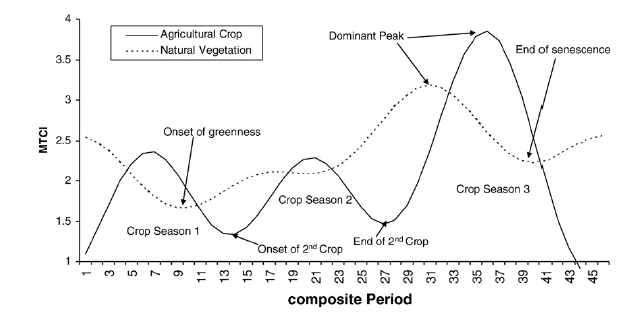
\includegraphics[width=\linewidth]{Images-phenology-fda/PhenoVars_Jegan.png} \caption{Diagram illustrating typical phenology patterns for agricultural land and natural vegetation from \cite{Dash:2010kva}. } \label{fig:phenology diagram} 
\end{figure}



\begin{figure}
	[htbp] \centering 
	\includegraphics[width=0.49\linewidth]{Images-phenology-fda/Satellite/India-current.png} 
	\includegraphics[width=0.49\linewidth]{Images-phenology-fda/Satellite/India-5-12-2000.png} \caption{Satellite image of study region in souther India from 2014 (left) and 2000 (right).} \label{fig:india} 
\end{figure}

\begin{figure}
	[htbp] \centering 
	\includegraphics[width=\linewidth]{Images-phenology-fda/land_cover.pdf} \caption{Land cover classification at 4.6~km spatial resolution derived from GLC2000 land cover database} \label{fig:land cover} 
\end{figure}

\begin{figure}
	[htbp] \centering 
	\includegraphics[width=\linewidth]{Images-phenology-fda/mean_by_LC_facet_year.pdf} \caption{Smoothed MTCI values by year and by land cover.} \label{fig:mean by LC} 
\end{figure}

\begin{figure}
	[htbp] \centering 
	\includegraphics[width=\linewidth]{Images-phenology-fda/Plots/landcover_ag_veg.pdf} \caption{Land cover map of the study region aggregated into ``Agriculture'', ``Vegetation'', and ``other''. Grid cells were labeled ``Vegetation'' if their original land cover was Tropical Evergreen, Subtropical Evergreen, Tropical Semievergreen, Tropical Moist Deciduous, or Coastal vegetation. Grid cells were labeled ``Agriculture'' is their original land cover was Rainfed Agriculture, Slope Agriculture, Irrigated Agriculture, or Irrigated Intensive Agriculture. Black dots show the location of homogeneous agriculture grid cells.} \label{fig:land cover ag vs. veg} 
\end{figure}
\begin{figure}
	[htbp] \centering 
	\includegraphics[width=\linewidth]{Images-phenology-fda/Plots/proportion_agriculture.pdf} \caption{Map of the study region showing the proportion of agricultural land within each of the 4.6~km$\times$4.6~km grid cells based on the GLC2000 land cover database. } \label{fig:proportion agriculture} 
\end{figure}

% \begin{figure}
% 	[htbp] \centering
% 	\includegraphics[width=\linewidth]{Images-phenology-fda/ag_hom_cells.pdf} \caption{Map of the study region showing the location of homogeneous agriculture grid cells. } \label{fig:homogeneous ag cells}
% \end{figure}

\begin{figure}
	[htbp] \centering 
	\includegraphics[width=\linewidth]{Images-phenology-fda/hom_curves_agriculture_east_west_2003_2.pdf} \caption{Observed MCTI values for homogeneous agriculture cells in 2003. The color identified curves as either in the eastern or western part of the country. The homogeneous agriculture cells on the west side of the country consist of intensely irrigated agriculture. } \label{fig:ag cell east vs west} 
\end{figure}


% section data (end)
\section{Methodology} 
% (fold)
\label{sec:methodology}

The data have both a rich spatial and temporal component. We view the data as a collection of curves that are each a function of time, but have the attribute of a spatial location. The map in Figure \ref{fig:land cover} consists of many different land cover types largely separated on the east and west by agricultural land and natural vegetation, respectively. Our primary interest is to be able to detect locations that are possibly misclassified as natural vegetation. Our general approach consists of the following steps:
\begin{itemize}
	\item Label each cell as either vegetation, agriculture, or other. Figure \ref{fig:land cover ag vs. veg} shows the land cover map using this labeling.
	\item Construct a set of empirical basis functions derived from land that is primarily agricultural. We only include homogeneous agriculture cells defined to be cells with 100\% agricultural land cover according to the proportions derived from the GLC2000 database. Figure \ref{fig:proportion agriculture} shows the proportion of agricultural land based on GLC2000 database, and Figure \ref{fig:homogeneous ag cells} shows the location of the homogeneous agricultural cells. The homogeneous agriculture cells on the western side of the country are irrigation intensive agriculture and exhibit different phenological patterns than agriculture cells on the eastern part of the country as can be seen in Figure \ref{fig:ag cell east vs west}. For this reason we did not include these locations in the set of homogeneous agriculture locations. 
	\item Project all of the data onto the basis, reducing the information for each curve to a low dimensional vector of coefficients.
	\item Construct a classifier for the coefficient vectors by using a training set corresponding to the homogeneous agriculture locations and an equal number of homogeneous vegetation locations.  
\end{itemize}

\subsection{Functional model for homogeneous grid cells} % (fold)
\label{sub:subsection_name}

 For the set of homogeneous agricultural grid cells we model the phenological trajectories $X(t)$ as a continuos second order stochastic process with mean $\mu(t)$ and bivariate temporal covariance function
\[ C_{0}(s,t)=E([X(s)-E(X(s))][X(t)-E(X(t))]),\mbox{ }\forall s,t\in \T. \]
We analyze the process on an annual basis which for the 8-day composite MCTI values corresponds to the time domain $\T = [0,46]$, but in what follows the data are rescaled to the interval $[0,1]$. We assume the underling trajectories $X(\cdot)$ are smooth in that they take values in a reproducing kernel Hilbert space $\H= \{f : f, f' \mbox{ absolutely continuous}, f'' \in L_2[0,1]\}$. 

Let $\{X_{1},X_{2},\dots,X_{N}\}$ represent the collection of realizations of $X$, and we consider the following model for the observed MCTI values $Y_{ij}$,
\[ Y_{ij}=X_{i}(t_{ij})+\epsilon_{ij},\mbox{ }j=1,\dots,46;\mbox{ }i=1,\dots,N, \]
where $i$ indexes the centroid of the spatial grid cell and $j$ indexes the sampling times corresponding to the 8-day composite MTCI values. The $\epsilon_{ij}$ are independently and identically distributed measurement errors with mean zero and finite variance $\sigma_{0}^{2}.$ It is further assumed that the random functions $X$, and measurement errors $\epsilon$ are mutually independent. 
% subsection subsection_name (end)

\subsection{Smoothing} 

% (fold)
\label{sub:smoothing}
We achieve smooth versions of the observed curves by expressing them as a finite basis expansion of principal component functions corresponding the the covariance function $C_0(s,t)$. The covariance of the observed process $Y_{ij}$ is given by
\begin{equation}
	C(Y_i(t_j), Y_i(t_k)) = C_0(X_i(t_j), X_i(t_k)) + \sigma^2_0 \delta_{jk}
\end{equation}
where $\delta_{jk}$ equals 1 if $j=k$ and is equal to zero otherwise. The covariance function $C_0(s,t)$ is recovered by performing bivariate smoothing on the sample covariance omitting the diagonal values. The methodology, which is described in detail in described in Chapter \ref{ch:covariance estimation}, achieves both efficient estimation of $C_0(s,t)$ and results in closed-form estimates of corresponding principal component functions. By assuming the trajectories $X$ belong to a reproducing kernel Hilbert space is has been shown to have optimal convergence properties due to the fact that the covariance function necessarily resides in the tensor product space $\H\tprod\H$. This fact motivates the following covariance function estimator.

Let $\mathbf{b}^{(i)} = [(Y_{ij}-\mu(t_{ij}))(Y_{ij'}-\mu(t_{ij'}))]_{1\leq j\neq j'\leq 46}$, $i=1, \dots, N$. Further, let
\[ \mathbf{b} = (\mathbf{b}^{(1)T}, \mathbf{b}^{(2)T}, \dots, \mathbf{b}^{(n)T} )^T, \]
where the vectors $\mathbf{b}^{(i)}$ contain all pairwise products of observations on the $i$th curve, excluding those that are the product of an observation with itself which correspond to the diagonal values on $[0,1]\times [0,1]$. Using this notation the covariance estimator corresponds to the following optimization problem,
\begin{equation}
	 \widehat{C}_{\lambda}=\stackrel[C \in \H\otimes \H]{}{\text{ argmin}} \left\{\frac{1}{n46^2-n46} (\mathbf{b} - \mathbf{C})^T(\mathbf{b} - \mathbf{C})+\lambda\left\Vert C\right\Vert _{\breve{\H}}^{2} \right\},
	 \label{pheno: cov est}
	 \end{equation}
where
\[ \mathbf{C} = [C(t_{i,j}, t_{i'j'})] \]
and $\lambda$ is a smoothing parameter estimated using cross validation.

In order to account for possible spatial correlation between curves we apply the weighting scheme developed in Chapter \ref{ch:functional kriging}. In Section \ref{sub:weighted covariance} we showed that we can achieve significant improvements in covariance estimation by down weighting curves corresponding to high location density areas.

We proceed to define location intensity as the number of locations per unit area and denote location intensity at location $i$ by $\gamma_i$.  The following weight function provides a simple yet flexible way to construct weights,
\begin{equation}
	w_i = \left(\frac{1}{\gamma_i}\right)^p. \label{pheno:weight function}
\end{equation}
The weight function \eqref{pheno:weight function} includes a scaling parameter, $p$, whose appropriate value depends on the degree of spatial dependence in the data. In the section \ref{sub:selecting_an_appropriate_weight} we describe how to investigate possible values for $p$.


Let $\mathbf{W} = diag(\mathbf{w}_1, \dots, \mathbf{w}_n)$, where $\mathbf{w}_i$ is a row vector whose length is equal to the length of $\mathbf{b}^{(i)}$ and whose components are all equal to $w_i$. The spatially re-weighted covariance estimator is constructed by replacing the loss function in \ref{pheno: cov est} with 
\begin{equation}
	l(C)= (\mathbf{b} - \mathbf{C})^T\mathbf{W}(\mathbf{b} - \mathbf{C}). \label{pheno:diag weighted loss function} 
\end{equation}
Details of the estimation of $\widehat{C(s,t)}$ and its corresponding eigenfunctions $\hat{\psi}_k(t)$ are described in Chapter \ref{ch:covariance estimation}. 

To produce smooth estimates of the trajectories $X_i(t)$, project the observations $Y_i(t_j), j = 1, \dots, 46$ onto the finite dimensional functional basis $\{\hat{\psi}_k(t), k = 1, \dots, q\}$, where $q$ is chosen such that at least $90\%$ of the variation is explained. The fitted trajectories admit the following representation
\begin{equation}
	\widehat{X_i(t)} = \sum_{k=1}^q\alpha_{k,i} \hat{\psi}_k(t) = \boldsymbol{\alpha_i'}\boldsymbol{\psi}.
	\label{phen:coef}
\end{equation}
In this representation the randomness associated with each random trajectory $X(t)$ is captured in the coefficient vector $\boldsymbol{\alpha}$. This allows one to take advantage the vast methods available for multivariate data. In this work we use linear discriminant analysis to classify land cover, but this framework allows for many possibilities for using multivariate methods for functional data analysis. 
\subsubsection{Selecting an appropriate weight} 

% (fold)
\label{sub:selecting_an_appropriate_weight} 
Selection of the weight parameter $p$ in \eqref{pheno:weight function} is a challenging problem as the optimal choice fundamentally depends on the strength of dependence in the data. However, simulations presented in Chapter \ref{ch:functional kriging} indicate that precision in estimating the value of $p$ is not necessary by observing that values between 1/3 and 1/2 are suitable for varying levels of spatial dependence. We performed a similar simulation study using the same framework, but using locations corresponding to the homogeneous agriculture grid cells. The simulation results using the homogeneous agriculture locations were consistent with the results in Chapter \ref{ch:functional kriging}. Based on these results we used $p=1/2$ to define the weights. The locations and their weights derived from \eqref{pheno:weight function} using $p=1/2$ are shown in Figure \ref{fig:india weighted locs}. 
\begin{figure}
	[h] \centering 
	\includegraphics[width=0.7\linewidth]{Images-phenology-fda/india_wt_locs.pdf} \caption{Spatial locations of the homogeneous agricultural grid cells. The size of the point indicates the weight used for data at that location for estimating the covariance function. } \label{fig:india weighted locs} 
\end{figure}


% subsection selecting_an_appropriate_weight (end)
% subsection smoothing (end)
\subsection{Land Cover Classification} 
 % (fold)
\label{sub:land_cover_classification}

The representation of each curve in terms of the FPC expansion \eqref{phen:coef} associates to each trajectory a set of $q$ coefficients. The dimension reduction achieved with this representation allows one to bring to bare any number of classical statistical methods---which is the major benefit of this approach. We describe a method for classification suitable for this type of data structure motivated by the phenological application as follows.

%We describe two methods for classification suitable for this type of data structure, one using linear discriminant analysis and one using logistic regression motivated by the phenological application as follows. 

\subsubsection{Linear Discriminant Analysis} % (fold)
\label{sub:LDA}
Linear discrimant analysis is a popular method in the class of linear classifiers; here the term linear referes to the structure of the decision boundary. Let $\mathcal{C} = \{ \text{Agriculture}, \text{Vegetation}\}$ be the set of all possible classes, and let C be a random variable taking values in $\mathcal{C}$. The classification decision is based on the rule
\begin{equation}
	\hat{\text{C}}(\boldsymbol{\alpha}) = 
	\begin{cases}
			\text{Agriculture} \hfill & \text{ if } \text{Pr}(\text{C = Agriculture }| \boldsymbol{\alpha})> \text{Pr}(\text{C = Vegetation }| \boldsymbol{\alpha})\\
			\text{Vegetation} \hfill & \text{ otherwise}
	\end{cases}
\end{equation}  
Computation of the posterior probabilities follows from modeling the class-conditional densities $f_k(\boldsymbol\alpha)$ as multivariate Gaussian distributions
\begin{equation}
	f_k(\boldsymbol\alpha) = \frac{1}{(2\pi)^{p/2}}e^{-\frac{1}{2}(\boldsymbol\alpha - \boldsymbol\mu_k)^T\Sigma^{-1}(\boldsymbol\alpha - \boldsymbol\mu_k)}
\end{equation}
and the assumption in LDA is a common covariance matrix between classes. With this assumption 
\begin{equation}
	\text{Pr}(\text{C} = \text{Agriculture } | \boldsymbol\alpha) = \frac{f_{ag}(\boldsymbol\alpha)\pi_{ag}}{f_{ag}(\boldsymbol\alpha)\pi_{ag}+f_{veg}(\boldsymbol\alpha)\pi_{veg}}
\end{equation}
where $\pi_{ag}$ and $\pi_{veg}$ are the prior probabilities class membership. Training data are used to estimate all parameters using maximum likelihood. The strong distributional assumptions make this approach computationally efficient, but diagnostics should be used to check if the assumption of multivariate Gaussian distributions with common covariance structure is reasonable. 
 % subsection LDA (end)

% \subsubsection{Logistic Regression} % (fold)
% \label{sub:subsection_name}
%
% % subsection subsection_name (end)
% The coefficient vectors are low dimensional and can be used effectively as covariates because colinearity is mitigated by the used of FPCs. We describe an approach for classification using a logistic regression model.
%
% Let $Z_i$ be a random variable connected to the land cover class of spatial grid cell location $i$, which takes values in $\{0,1\}$ corresponding the classes $\{$Vegetation, Agriculture$\}$. Logistic regression is a special case of a generalized linear model whose random component is modeled as a Bernoulli distribution and whose link function is logit(p),
% \begin{equation}
% 	Z_i | \alpha_{1,i}, \dots, \alpha_{4,i} \sim \text{Bernoulli}(p_i) \nonumber
% \end{equation}
% and
% \begin{equation}
% 	ln \left(\frac{p_i}{1-p_i}\right) = \beta_0 + \beta_1 \alpha_{1,i} + \dots + \beta_4 \alpha_{4,i}.\nonumber
% \end{equation}
% The fitted values $\hat{p_i} = \text{E}[Z_i| \alpha_{1,i}, \dots, \alpha_{4,i} ]$ are estimates of the probably that location $i$ has an agriculturally dominant land cover. The classifier we use follows the rule
% \begin{equation}
% 	\text{land cover}_i =
% 	\begin{cases}
% 			\text{Agriculture} \hfill & \text{ if $\hat{p}_i >= 1/2$}\\
% 			\text{Vegetation} \hfill & \text{ if $\hat{p}_i < 1/2$}
% 	\end{cases}
% 	\nonumber
% \end{equation}



% subsection land_cover_classification (end)
% section methodology (end)
\section{Results} 
% (fold)
For each year function principal components were computed and for all years only three FPCs were needed to account for at least 90\% of the variation based on the eigenvalues. The first three FPCs for each year are shown in Figure \ref{fig:pcf all years}. These functions and a constant function were used as basis functions which were fit to all locations. The classification results are shown in Figures \ref{fig:misclassified vegetation} and \ref{fig:misclassified agriculture}, where only discrepancies in classification between the classifier proposed in this work and the GLC2000 classification are shown with highlighted red cells. Figure \ref{fig:misclassified vegetation} indicates and extensive area in the northern part of the study region that is being classified as agriculture by the LDA classifier, but is labeled as natural vegetion using the GLC2000 data base. 

Figures \ref{partimat 2003}, \ref{partimat 2004},\ref{partimat 2005},\ref{partimat 2006}, and \ref{partimat 2007} show LDA estimates for all unique pairs of variables with colors highlighting the linear decision boundary. These Figures indicate that the model assumptions are not a concern in this case, and that a linear decision boundary is likely sufficient for these data. 

\begin{figure}
	[htbp] \centering 
	\includegraphics[width=\linewidth]{Images-phenology-fda/PCF_all_years.pdf} \caption{First three principal component functions computed for each year from 2003-2007. } \label{fig:pcf all years} 
\end{figure}

\begin{figure}
	[htbp] \centering 
	\includegraphics[width=\linewidth]{Images-phenology-fda/Plots/misclassified_vegetation.pdf} \caption{Map of the study region showing locations where classification results differ from the original GLC2000 derived land classification. Locations that the GLC2000 identified as vegetation, but were classified as agricultural are shown in red.   } 
	\label{fig:misclassified vegetation} 
\end{figure}

\begin{figure}
	[htbp] \centering 
	\includegraphics[width=\linewidth]{Images-phenology-fda/Plots/misclassified_agriculture.pdf} \caption{Map of the study region showing locations where classification results differ from the original GLC2000 derived land classification. Locations that the GLC2000 identified as agriculture, but were classified as natural vegetation are shown in red.} 
	\label{fig:misclassified agriculture} 
\end{figure}

\begin{figure}
	[htbp] \centering 
	\includegraphics[width=\linewidth]{Images-phenology-fda/Plots/prob_ag.pdf} \caption{ Posterior probability of Agricultural land cover. } 
	\label{fig:probability map} 
\end{figure}


\label{sec:results}


% section results (end)
\section{Discussion} 
We have developed an approach to land cover classification between agricultural and natural vegetation using observe MTCI data. The classification maps shown in Figure \ref{fig:classification map} indicate that a large number of locations that the GLC2000 based classification labelled as natural vegetation are being classified as agriculture. Many of the discrepancies are along the center ridge of where it is not surprising to see conflicting classifications as this is where the agricultural east converges with the tropical west; however there are two areas within on the west side of the country that seem to be consistently classified as agricultural: a large area toward the northern border of the region, and a small grouping of cells near the middle of the western side of the country. 

Satellite imagery sheds some light on what might be causing this effect. Figure \ref{fig:north india} shows a zoomed in satellite image of the northern area of the region both in the year 2000 and in 2003. There appears to be large area of possible deforested land that is much more apparent in 2003 than it is the satellite picture from 2000. Figure \ref{fig:north india zoom} shows a high resolution image of the deforested area. This finding shows that the classification method is effective at detecting anthropomorphic changes in vegetation land cover using the MTCI data. 

The map in Figure \ref{fig:proportion agriculture} shows the proportion of agricultural land in each grid cell based on the GLC2000 database. This map indicates that some cells in the two regions we have identified had some agricultural land cover according to the GLC2000 database, but not to the spatial extent that we observe in the MTCI classification. That is, many of the grid cells consistently classified as agriculture by the MTCI classification have near zero proportion of agricultural land according to the GLC2000 database. This suggests an actual change over time (since 2000) of land cover in these areas which could correspond to increased deforestation, increased agriculture development, or both. 

The results do not necessarily indicate an increase of agricultural land over time, as the classification is not completely consistent over time in many areas. For example, it is 2003 where the most vegetation land is classified as agriculture. This may indicate that mixed land cover cells exhibit the behavior of natural vegetation or agriculture depending on the year. The point, however, is not to say these cells \emph{are} agricultural or \emph{are} natural vegetation, but to recognize that they are neither and should be given careful consideration---and possibly omitted---for analyses that seek to characterize phenological variables with respect to land cover. 


% (fold)
\label{sec:discussion}
\begin{figure}
	[htbp] \centering 
	\includegraphics[width=0.7\linewidth]{Images-phenology-fda/Satellite/India-2000.png} \\[1cm]
	\includegraphics[width=0.7\linewidth]{Images-phenology-fda/Satellite/India-10-10-2003.png} \\
	\caption{Satellite image of northwestern part of the study region in southern India from 2000 (top) and 2003 (bottom). } 
	
	\label{fig:north india} 
\end{figure}
\begin{figure}
	[htbp] \centering 
	\includegraphics[width=0.7\linewidth]{Images-phenology-fda/Satellite/India-12-29-2003.png} \caption{Satellite image of study region in souther India showing an area of possible deforestation and agricultural development.} 
	\label{fig:north india zoom} 
\end{figure}
% section conclusion (end)

\section{Supplementary Material} % (fold)
\label{sec:supplementary_material}

\begin{figure}
	[htbp] \centering 
	\includegraphics[width=0.8\linewidth]{Images-phenology-fda/Plots/partimat_2003.pdf} \caption{} 
	\label{partimat 2003} 
\end{figure}
\begin{figure}
	[htbp] \centering 
	\includegraphics[width=0.8\linewidth]{Images-phenology-fda/Plots/partimat_2004.pdf} \caption{} 
	\label{partimat 2004} 
\end{figure}
\begin{figure}
	[htbp] \centering 
	\includegraphics[width=0.8\linewidth]{Images-phenology-fda/Plots/partimat_2005.pdf} \caption{} 
	\label{partimat 2005} 
\end{figure}
\begin{figure}
	[htbp] \centering 
	\includegraphics[width=0.8\linewidth]{Images-phenology-fda/Plots/partimat_2006.pdf} \caption{} 
	\label{partimat 2006} 
\end{figure}
\begin{figure}
	[htbp] \centering 
	\includegraphics[width=0.8\linewidth]{Images-phenology-fda/Plots/partimat_2007.pdf} \caption{} 
	\label{partimat 2007} 
\end{figure}

% section supplementary_material (end)



